\documentclass[1p]{elsarticle_modified}
%\bibliographystyle{elsarticle-num}

%\usepackage[colorlinks]{hyperref}
%\usepackage{abbrmath_seonhwa} %\Abb, \Ascr, \Acal ,\Abf, \Afrak
\usepackage{amsfonts}
\usepackage{amssymb}
\usepackage{amsmath}
\usepackage{amsthm}
\usepackage{scalefnt}
\usepackage{amsbsy}
\usepackage{kotex}
\usepackage{caption}
\usepackage{subfig}
\usepackage{color}
\usepackage{graphicx}
\usepackage{xcolor} %% white, black, red, green, blue, cyan, magenta, yellow
\usepackage{float}
\usepackage{setspace}
\usepackage{hyperref}

\usepackage{tikz}
\usetikzlibrary{arrows}

\usepackage{multirow}
\usepackage{array} % fixed length table
\usepackage{hhline}

%%%%%%%%%%%%%%%%%%%%%
\makeatletter
\renewcommand*\env@matrix[1][\arraystretch]{%
	\edef\arraystretch{#1}%
	\hskip -\arraycolsep
	\let\@ifnextchar\new@ifnextchar
	\array{*\c@MaxMatrixCols c}}
\makeatother %https://tex.stackexchange.com/questions/14071/how-can-i-increase-the-line-spacing-in-a-matrix
%%%%%%%%%%%%%%%

\usepackage[normalem]{ulem}

\newcommand{\msout}[1]{\ifmmode\text{\sout{\ensuremath{#1}}}\else\sout{#1}\fi}
%SOURCE: \msout is \stkout macro in https://tex.stackexchange.com/questions/20609/strikeout-in-math-mode

\newcommand{\cancel}[1]{
	\ifmmode
	{\color{red}\msout{#1}}
	\else
	{\color{red}\sout{#1}}
	\fi
}

\newcommand{\add}[1]{
	{\color{blue}\uwave{#1}}
}

\newcommand{\replace}[2]{
	\ifmmode
	{\color{red}\msout{#1}}{\color{blue}\uwave{#2}}
	\else
	{\color{red}\sout{#1}}{\color{blue}\uwave{#2}}
	\fi
}

\newcommand{\Sol}{\mathcal{S}} %segment
\newcommand{\D}{D} %diagram
\newcommand{\A}{\mathcal{A}} %arc


%%%%%%%%%%%%%%%%%%%%%%%%%%%%%5 test

\def\sl{\operatorname{\textup{SL}}(2,\Cbb)}
\def\psl{\operatorname{\textup{PSL}}(2,\Cbb)}
\def\quan{\mkern 1mu \triangleright \mkern 1mu}

\theoremstyle{definition}
\newtheorem{thm}{Theorem}[section]
\newtheorem{prop}[thm]{Proposition}
\newtheorem{lem}[thm]{Lemma}
\newtheorem{ques}[thm]{Question}
\newtheorem{cor}[thm]{Corollary}
\newtheorem{defn}[thm]{Definition}
\newtheorem{exam}[thm]{Example}
\newtheorem{rmk}[thm]{Remark}
\newtheorem{alg}[thm]{Algorithm}

\newcommand{\I}{\sqrt{-1}}
\begin{document}

%\begin{frontmatter}
%
%\title{Boundary parabolic representations of knots up to 8 crossings}
%
%%% Group authors per affiliation:
%\author{Yunhi Cho} 
%\address{Department of Mathematics, University of Seoul, Seoul, Korea}
%\ead{yhcho@uos.ac.kr}
%
%
%\author{Seonhwa Kim} %\fnref{s_kim}}
%\address{Center for Geometry and Physics, Institute for Basic Science, Pohang, 37673, Korea}
%\ead{ryeona17@ibs.re.kr}
%
%\author{Hyuk Kim}
%\address{Department of Mathematical Sciences, Seoul National University, Seoul 08826, Korea}
%\ead{hyukkim@snu.ac.kr}
%
%\author{Seokbeom Yoon}
%\address{Department of Mathematical Sciences, Seoul National University, Seoul, 08826,  Korea}
%\ead{sbyoon15@snu.ac.kr}
%
%\begin{abstract}
%We find all boundary parabolic representation of knots up to 8 crossings.
%
%\end{abstract}
%\begin{keyword}
%    \MSC[2010] 57M25 
%\end{keyword}
%
%\end{frontmatter}

%\linenumbers
%\tableofcontents
%
\newcommand\colored[1]{\textcolor{white}{\rule[-0.35ex]{0.8em}{1.4ex}}\kern-0.8em\color{red} #1}%
%\newcommand\colored[1]{\textcolor{white}{ #1}\kern-2.17ex	\textcolor{white}{ #1}\kern-1.81ex	\textcolor{white}{ #1}\kern-2.15ex\color{red}#1	}

{\Large $\underline{12n_{0312}~(K12n_{0312})}$}

\setlength{\tabcolsep}{10pt}
\renewcommand{\arraystretch}{1.6}
\vspace{1cm}\begin{tabular}{m{100pt}>{\centering\arraybackslash}m{274pt}}
\multirow{5}{120pt}{
	\centering
	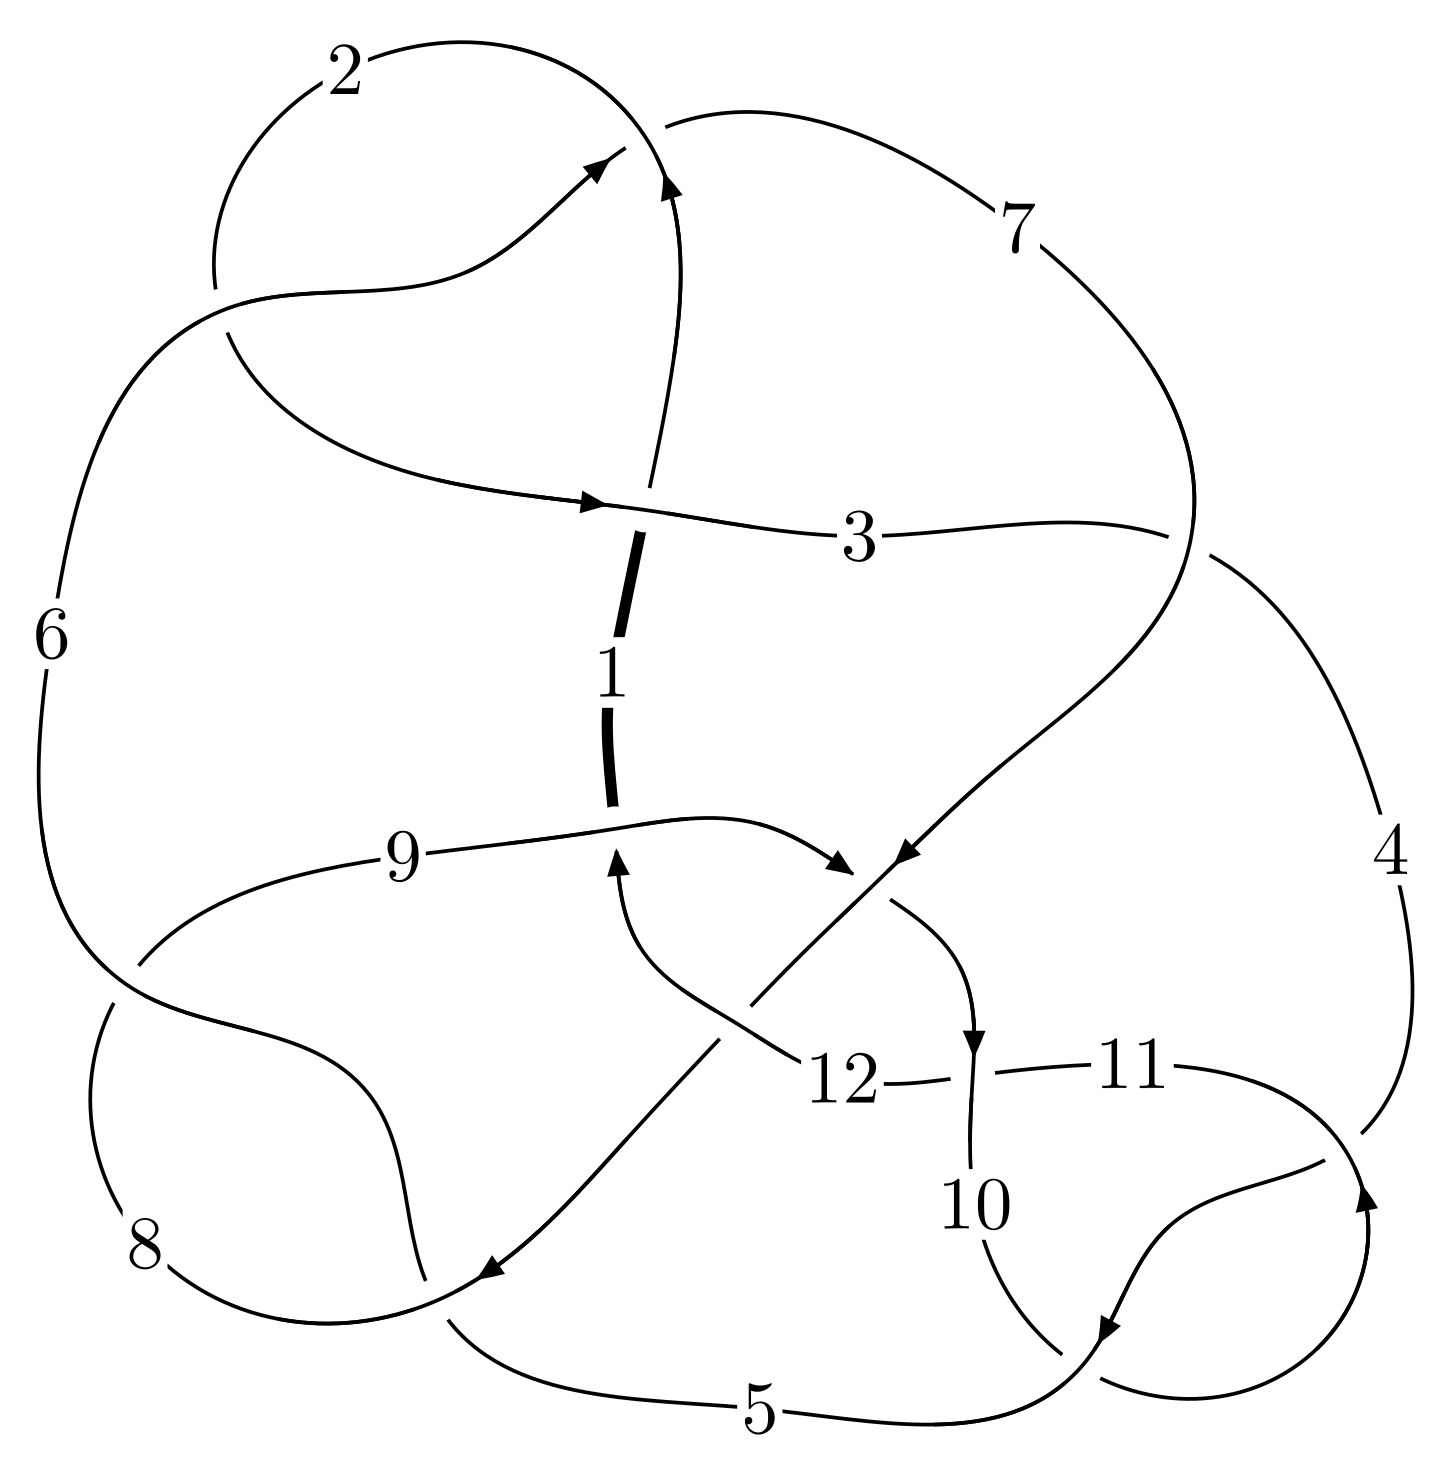
\includegraphics[width=112pt]{../../../GIT/diagram.site/Diagrams/png/2401_12n_0312.png}\\
\ \ \ A knot diagram\footnotemark}&
\allowdisplaybreaks
\textbf{Linearized knot diagam} \\
\cline{2-2}
 &
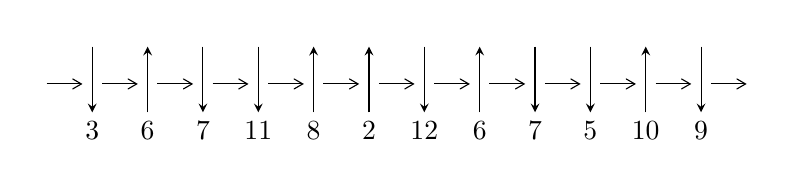
\begin{tikzpicture}[x=20pt, y=17pt]
	% nodes
	\node (C0) at (0, 0) {};
	\node (C1) at (1, 0) {};
	\node (C1U) at (1, +1) {};
	\node (C1D) at (1, -1) {3};

	\node (C2) at (2, 0) {};
	\node (C2U) at (2, +1) {};
	\node (C2D) at (2, -1) {6};

	\node (C3) at (3, 0) {};
	\node (C3U) at (3, +1) {};
	\node (C3D) at (3, -1) {7};

	\node (C4) at (4, 0) {};
	\node (C4U) at (4, +1) {};
	\node (C4D) at (4, -1) {11};

	\node (C5) at (5, 0) {};
	\node (C5U) at (5, +1) {};
	\node (C5D) at (5, -1) {8};

	\node (C6) at (6, 0) {};
	\node (C6U) at (6, +1) {};
	\node (C6D) at (6, -1) {2};

	\node (C7) at (7, 0) {};
	\node (C7U) at (7, +1) {};
	\node (C7D) at (7, -1) {12};

	\node (C8) at (8, 0) {};
	\node (C8U) at (8, +1) {};
	\node (C8D) at (8, -1) {6};

	\node (C9) at (9, 0) {};
	\node (C9U) at (9, +1) {};
	\node (C9D) at (9, -1) {7};

	\node (C10) at (10, 0) {};
	\node (C10U) at (10, +1) {};
	\node (C10D) at (10, -1) {5};

	\node (C11) at (11, 0) {};
	\node (C11U) at (11, +1) {};
	\node (C11D) at (11, -1) {10};

	\node (C12) at (12, 0) {};
	\node (C12U) at (12, +1) {};
	\node (C12D) at (12, -1) {9};
	\node (C13) at (13, 0) {};

	% arrows
	\draw[->,>={angle 60}]
	(C0) edge (C1) (C1) edge (C2) (C2) edge (C3) (C3) edge (C4) (C4) edge (C5) (C5) edge (C6) (C6) edge (C7) (C7) edge (C8) (C8) edge (C9) (C9) edge (C10) (C10) edge (C11) (C11) edge (C12) (C12) edge (C13) ;	\draw[->,>=stealth]
	(C1U) edge (C1D) (C2D) edge (C2U) (C3U) edge (C3D) (C4U) edge (C4D) (C5D) edge (C5U) (C6D) edge (C6U) (C7U) edge (C7D) (C8D) edge (C8U) (C9U) edge (C9D) (C10U) edge (C10D) (C11D) edge (C11U) (C12U) edge (C12D) ;
	\end{tikzpicture} \\
\hhline{~~} \\& 
\textbf{Solving Sequence} \\ \cline{2-2} 
 &
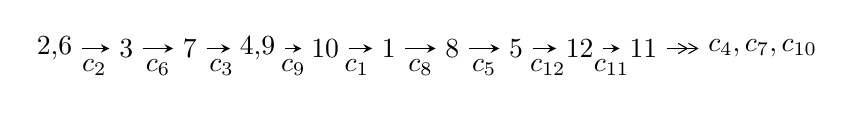
\begin{tikzpicture}[x=23pt, y=7pt]
	% node
	\node (A0) at (-1/8, 0) {2,6};
	\node (A1) at (1, 0) {3};
	\node (A2) at (2, 0) {7};
	\node (A3) at (49/16, 0) {4,9};
	\node (A4) at (33/8, 0) {10};
	\node (A5) at (41/8, 0) {1};
	\node (A6) at (49/8, 0) {8};
	\node (A7) at (57/8, 0) {5};
	\node (A8) at (65/8, 0) {12};
	\node (A9) at (73/8, 0) {11};
	\node (C1) at (1/2, -1) {$c_{2}$};
	\node (C2) at (3/2, -1) {$c_{6}$};
	\node (C3) at (5/2, -1) {$c_{3}$};
	\node (C4) at (29/8, -1) {$c_{9}$};
	\node (C5) at (37/8, -1) {$c_{1}$};
	\node (C6) at (45/8, -1) {$c_{8}$};
	\node (C7) at (53/8, -1) {$c_{5}$};
	\node (C8) at (61/8, -1) {$c_{12}$};
	\node (C9) at (69/8, -1) {$c_{11}$};
	\node (A10) at (11, 0) {$c_{4},c_{7},c_{10}$};

	% edge
	\draw[->,>=stealth]	
	(A0) edge (A1) (A1) edge (A2) (A2) edge (A3) (A3) edge (A4) (A4) edge (A5) (A5) edge (A6) (A6) edge (A7) (A7) edge (A8) (A8) edge (A9) ;
	\draw[->>,>={angle 60}]	
	(A9) edge (A10);
\end{tikzpicture} \\ 

\end{tabular} \\

\footnotetext{
The image of knot diagram is generated by the software ``\textbf{Draw programme}" developed by Andrew Bartholomew(\url{http://www.layer8.co.uk/maths/draw/index.htm\#Running-draw}), where we modified some parts for our purpose(\url{https://github.com/CATsTAILs/LinksPainter}).
}\phantom \\ \newline 
\centering \textbf{Ideals for irreducible components\footnotemark of $X_{\text{par}}$} 
 
\begin{align*}
I^u_{1}&=\langle 
-5.27353\times10^{50} u^{39}+5.95554\times10^{50} u^{38}+\cdots+5.81254\times10^{51} b+4.59993\times10^{51},\\
\phantom{I^u_{1}}&\phantom{= \langle  }7.75948\times10^{50} u^{39}-3.86755\times10^{51} u^{38}+\cdots+5.81254\times10^{51} a-9.39756\times10^{51},\;u^{40}-2 u^{39}+\cdots+7 u+1\rangle \\
I^u_{2}&=\langle 
2 u^{14}- u^{13}+8 u^{12}-5 u^{11}+19 u^{10}-13 u^9+27 u^8-16 u^7+28 u^6-9 u^5+20 u^4+u^3+10 u^2+b+2 u+2,\\
\phantom{I^u_{2}}&\phantom{= \langle  }u^{15}-2 u^{14}+\cdots+a-2,\;u^{16}- u^{15}+\cdots- u+1\rangle \\
\\
\end{align*}
\raggedright * 2 irreducible components of $\dim_{\mathbb{C}}=0$, with total 56 representations.\\
\footnotetext{All coefficients of polynomials are rational numbers. But the coefficients are sometimes approximated in decimal forms when there is not enough margin.}
\newpage
\renewcommand{\arraystretch}{1}
\centering \section*{I. $I^u_{1}= \langle -5.27\times10^{50} u^{39}+5.96\times10^{50} u^{38}+\cdots+5.81\times10^{51} b+4.60\times10^{51},\;7.76\times10^{50} u^{39}-3.87\times10^{51} u^{38}+\cdots+5.81\times10^{51} a-9.40\times10^{51},\;u^{40}-2 u^{39}+\cdots+7 u+1 \rangle$}
\flushleft \textbf{(i) Arc colorings}\\
\begin{tabular}{m{7pt} m{180pt} m{7pt} m{180pt} }
\flushright $a_{2}=$&$\begin{pmatrix}1\\0\end{pmatrix}$ \\
\flushright $a_{6}=$&$\begin{pmatrix}0\\u\end{pmatrix}$ \\
\flushright $a_{3}=$&$\begin{pmatrix}1\\- u^2\end{pmatrix}$ \\
\flushright $a_{7}=$&$\begin{pmatrix}u\\u\end{pmatrix}$ \\
\flushright $a_{4}=$&$\begin{pmatrix}u^4+u^2+1\\u^4\end{pmatrix}$ \\
\flushright $a_{9}=$&$\begin{pmatrix}-0.133496 u^{39}+0.665380 u^{38}+\cdots+15.0043 u+1.61677\\0.0907267 u^{39}-0.102460 u^{38}+\cdots+0.430261 u-0.791380\end{pmatrix}$ \\
\flushright $a_{10}=$&$\begin{pmatrix}-0.224885 u^{39}+0.863520 u^{38}+\cdots+12.9927 u+1.29738\\-0.000662998 u^{39}+0.0956792 u^{38}+\cdots-1.58129 u-1.11078\end{pmatrix}$ \\
\flushright $a_{1}=$&$\begin{pmatrix}u^2+1\\- u^4\end{pmatrix}$ \\
\flushright $a_{8}=$&$\begin{pmatrix}-0.133496 u^{39}+0.665380 u^{38}+\cdots+15.0043 u+1.61677\\-0.100609 u^{39}+0.340183 u^{38}+\cdots-2.22497 u-1.18977\end{pmatrix}$ \\
\flushright $a_{5}=$&$\begin{pmatrix}1.39954 u^{39}-3.02014 u^{38}+\cdots+26.1706 u+4.28089\\0.281992 u^{39}-0.623894 u^{38}+\cdots+2.36583 u+0.204479\end{pmatrix}$ \\
\flushright $a_{12}=$&$\begin{pmatrix}-0.0433203 u^{39}+0.378199 u^{38}+\cdots+15.8786 u+2.05202\\0.483864 u^{39}-1.27646 u^{38}+\cdots-0.426089 u-1.03092\end{pmatrix}$ \\
\flushright $a_{11}=$&$\begin{pmatrix}-2.08778 u^{39}+5.36211 u^{38}+\cdots-10.8586 u-2.03985\\-0.147373 u^{39}+0.395336 u^{38}+\cdots-2.10105 u-0.958378\end{pmatrix}$\\&\end{tabular}
\flushleft \textbf{(ii) Obstruction class $= -1$}\\~\\
\flushleft \textbf{(iii) Cusp Shapes $= 4.30999 u^{39}-10.1429 u^{38}+\cdots+42.2706 u+1.05077$}\\~\\
\newpage\renewcommand{\arraystretch}{1}
\flushleft \textbf{(iv) u-Polynomials at the component}\newline \\
\begin{tabular}{m{50pt}|m{274pt}}
Crossings & \hspace{64pt}u-Polynomials at each crossing \\
\hline $$\begin{aligned}c_{1}\end{aligned}$$&$\begin{aligned}
&u^{40}+6 u^{39}+\cdots+23 u+1
\end{aligned}$\\
\hline $$\begin{aligned}c_{2},c_{6}\end{aligned}$$&$\begin{aligned}
&u^{40}-2 u^{39}+\cdots+7 u+1
\end{aligned}$\\
\hline $$\begin{aligned}c_{3}\end{aligned}$$&$\begin{aligned}
&u^{40}+5 u^{39}+\cdots+5688833 u+456713
\end{aligned}$\\
\hline $$\begin{aligned}c_{4},c_{10}\end{aligned}$$&$\begin{aligned}
&u^{40}+13 u^{38}+\cdots-4 u+7
\end{aligned}$\\
\hline $$\begin{aligned}c_{5},c_{8}\end{aligned}$$&$\begin{aligned}
&u^{40}+u^{39}+\cdots+4497 u+361
\end{aligned}$\\
\hline $$\begin{aligned}c_{7}\end{aligned}$$&$\begin{aligned}
&u^{40}+3 u^{39}+\cdots-4 u+1
\end{aligned}$\\
\hline $$\begin{aligned}c_{9}\end{aligned}$$&$\begin{aligned}
&u^{40}-5 u^{39}+\cdots-361724 u+608312
\end{aligned}$\\
\hline $$\begin{aligned}c_{11}\end{aligned}$$&$\begin{aligned}
&u^{40}-26 u^{39}+\cdots-362 u+49
\end{aligned}$\\
\hline $$\begin{aligned}c_{12}\end{aligned}$$&$\begin{aligned}
&u^{40}- u^{39}+\cdots-3750504 u+772753
\end{aligned}$\\
\hline
\end{tabular}\\~\\
\newpage\renewcommand{\arraystretch}{1}
\flushleft \textbf{(v) Riley Polynomials at the component}\newline \\
\begin{tabular}{m{50pt}|m{274pt}}
Crossings & \hspace{64pt}Riley Polynomials at each crossing \\
\hline $$\begin{aligned}c_{1}\end{aligned}$$&$\begin{aligned}
&y^{40}+66 y^{39}+\cdots-193 y+1
\end{aligned}$\\
\hline $$\begin{aligned}c_{2},c_{6}\end{aligned}$$&$\begin{aligned}
&y^{40}+6 y^{39}+\cdots+23 y+1
\end{aligned}$\\
\hline $$\begin{aligned}c_{3}\end{aligned}$$&$\begin{aligned}
&y^{40}+123 y^{39}+\cdots+6314489480935 y+208586764369
\end{aligned}$\\
\hline $$\begin{aligned}c_{4},c_{10}\end{aligned}$$&$\begin{aligned}
&y^{40}+26 y^{39}+\cdots+362 y+49
\end{aligned}$\\
\hline $$\begin{aligned}c_{5},c_{8}\end{aligned}$$&$\begin{aligned}
&y^{40}-59 y^{39}+\cdots+134503 y+130321
\end{aligned}$\\
\hline $$\begin{aligned}c_{7}\end{aligned}$$&$\begin{aligned}
&y^{40}- y^{39}+\cdots+8 y+1
\end{aligned}$\\
\hline $$\begin{aligned}c_{9}\end{aligned}$$&$\begin{aligned}
&y^{40}+53 y^{39}+\cdots+1499383242864 y+370043489344
\end{aligned}$\\
\hline $$\begin{aligned}c_{11}\end{aligned}$$&$\begin{aligned}
&y^{40}-18 y^{39}+\cdots-40394 y+2401
\end{aligned}$\\
\hline $$\begin{aligned}c_{12}\end{aligned}$$&$\begin{aligned}
&y^{40}+77 y^{39}+\cdots-906264208390 y+597147199009
\end{aligned}$\\
\hline
\end{tabular}\\~\\
\newpage\flushleft \textbf{(vi) Complex Volumes and Cusp Shapes}
$$\begin{array}{c|c|c}  
\text{Solutions to }I^u_{1}& \I (\text{vol} + \sqrt{-1}CS) & \text{Cusp shape}\\
 \hline 
\begin{aligned}
u &= \phantom{-}0.262608 + 0.958166 I \\
a &= -0.189880 + 0.941685 I \\
b &= \phantom{-}0.00591 + 1.77956 I\end{aligned}
 & -0.43866 + 2.24384 I & -3.81906 - 5.12194 I \\ \hline\begin{aligned}
u &= \phantom{-}0.262608 - 0.958166 I \\
a &= -0.189880 - 0.941685 I \\
b &= \phantom{-}0.00591 - 1.77956 I\end{aligned}
 & -0.43866 - 2.24384 I & -3.81906 + 5.12194 I \\ \hline\begin{aligned}
u &= \phantom{-}0.926209 + 0.156398 I \\
a &= \phantom{-}0.217139 + 0.674278 I \\
b &= \phantom{-}0.392314 - 0.960986 I\end{aligned}
 & \phantom{-}2.50089 + 2.28563 I & \phantom{-}2.12764 - 2.97233 I \\ \hline\begin{aligned}
u &= \phantom{-}0.926209 - 0.156398 I \\
a &= \phantom{-}0.217139 - 0.674278 I \\
b &= \phantom{-}0.392314 + 0.960986 I\end{aligned}
 & \phantom{-}2.50089 - 2.28563 I & \phantom{-}2.12764 + 2.97233 I \\ \hline\begin{aligned}
u &= -0.415141 + 0.823170 I \\
a &= -0.510209 - 1.251400 I \\
b &= \phantom{-}0.404330 - 0.813064 I\end{aligned}
 & \phantom{-}4.59855 + 0.55508 I & \phantom{-}3.65213 + 0.54524 I \\ \hline\begin{aligned}
u &= -0.415141 - 0.823170 I \\
a &= -0.510209 + 1.251400 I \\
b &= \phantom{-}0.404330 + 0.813064 I\end{aligned}
 & \phantom{-}4.59855 - 0.55508 I & \phantom{-}3.65213 - 0.54524 I \\ \hline\begin{aligned}
u &= -0.709121 + 0.812210 I \\
a &= \phantom{-}0.656724 + 0.475234 I \\
b &= \phantom{-}0.73014 + 1.50996 I\end{aligned}
 & \phantom{-}4.83926 - 5.18733 I & \phantom{-}5.25176 + 6.54277 I \\ \hline\begin{aligned}
u &= -0.709121 - 0.812210 I \\
a &= \phantom{-}0.656724 - 0.475234 I \\
b &= \phantom{-}0.73014 - 1.50996 I\end{aligned}
 & \phantom{-}4.83926 + 5.18733 I & \phantom{-}5.25176 - 6.54277 I \\ \hline\begin{aligned}
u &= \phantom{-}0.319846 + 1.045980 I \\
a &= \phantom{-}0.260908 + 0.248366 I \\
b &= -0.336124 - 0.552993 I\end{aligned}
 & -1.70481 + 5.48650 I & -4.87092 - 6.70893 I \\ \hline\begin{aligned}
u &= \phantom{-}0.319846 - 1.045980 I \\
a &= \phantom{-}0.260908 - 0.248366 I \\
b &= -0.336124 + 0.552993 I\end{aligned}
 & -1.70481 - 5.48650 I & -4.87092 + 6.70893 I\\
 \hline 
 \end{array}$$\newpage$$\begin{array}{c|c|c}  
\text{Solutions to }I^u_{1}& \I (\text{vol} + \sqrt{-1}CS) & \text{Cusp shape}\\
 \hline 
\begin{aligned}
u &= \phantom{-}0.751933 + 0.494508 I \\
a &= \phantom{-}1.392250 + 0.221845 I \\
b &= \phantom{-}0.514073 - 0.795694 I\end{aligned}
 & \phantom{-}1.51098 + 1.78901 I & \phantom{-}0.82025 - 3.56687 I \\ \hline\begin{aligned}
u &= \phantom{-}0.751933 - 0.494508 I \\
a &= \phantom{-}1.392250 - 0.221845 I \\
b &= \phantom{-}0.514073 + 0.795694 I\end{aligned}
 & \phantom{-}1.51098 - 1.78901 I & \phantom{-}0.82025 + 3.56687 I \\ \hline\begin{aligned}
u &= -0.297122 + 0.826943 I \\
a &= -0.493050 + 0.530886 I \\
b &= -0.409100 - 0.824445 I\end{aligned}
 & -2.88688 - 1.42829 I & -8.07911 - 0.82991 I \\ \hline\begin{aligned}
u &= -0.297122 - 0.826943 I \\
a &= -0.493050 - 0.530886 I \\
b &= -0.409100 + 0.824445 I\end{aligned}
 & -2.88688 + 1.42829 I & -8.07911 + 0.82991 I \\ \hline\begin{aligned}
u &= \phantom{-}0.294371 + 0.826929 I \\
a &= \phantom{-}0.378431 + 0.565801 I \\
b &= \phantom{-}0.768928 + 0.890271 I\end{aligned}
 & -0.24576 + 1.84711 I & -2.38841 - 3.47069 I \\ \hline\begin{aligned}
u &= \phantom{-}0.294371 - 0.826929 I \\
a &= \phantom{-}0.378431 - 0.565801 I \\
b &= \phantom{-}0.768928 - 0.890271 I\end{aligned}
 & -0.24576 - 1.84711 I & -2.38841 + 3.47069 I \\ \hline\begin{aligned}
u &= -1.054610 + 0.435101 I \\
a &= -1.58864 + 0.59883 I \\
b &= -0.25725 - 1.66736 I\end{aligned}
 & \phantom{-}4.29616 - 5.85650 I & \phantom{-}5.18701 + 8.29672 I \\ \hline\begin{aligned}
u &= -1.054610 - 0.435101 I \\
a &= -1.58864 - 0.59883 I \\
b &= -0.25725 + 1.66736 I\end{aligned}
 & \phantom{-}4.29616 + 5.85650 I & \phantom{-}5.18701 - 8.29672 I \\ \hline\begin{aligned}
u &= \phantom{-}0.454261 + 1.183960 I \\
a &= \phantom{-}0.032608 + 0.790796 I \\
b &= \phantom{-}0.87425 + 1.29247 I\end{aligned}
 & -0.78848 + 2.37152 I & -2.00000 + 0. I\phantom{ +0.000000I} \\ \hline\begin{aligned}
u &= \phantom{-}0.454261 - 1.183960 I \\
a &= \phantom{-}0.032608 - 0.790796 I \\
b &= \phantom{-}0.87425 - 1.29247 I\end{aligned}
 & -0.78848 - 2.37152 I & -2.00000 + 0. I\phantom{ +0.000000I}\\
 \hline 
 \end{array}$$\newpage$$\begin{array}{c|c|c}  
\text{Solutions to }I^u_{1}& \I (\text{vol} + \sqrt{-1}CS) & \text{Cusp shape}\\
 \hline 
\begin{aligned}
u &= \phantom{-}1.12042 + 0.91969 I \\
a &= -1.129020 + 0.673147 I \\
b &= -0.30929 + 1.59265 I\end{aligned}
 & \phantom{-}16.0958 + 2.3517 I & \phantom{-0.000000 } 0 \\ \hline\begin{aligned}
u &= \phantom{-}1.12042 - 0.91969 I \\
a &= -1.129020 - 0.673147 I \\
b &= -0.30929 - 1.59265 I\end{aligned}
 & \phantom{-}16.0958 - 2.3517 I & \phantom{-0.000000 } 0 \\ \hline\begin{aligned}
u &= -1.04883 + 1.00662 I \\
a &= -0.943173 - 0.988165 I \\
b &= \phantom{-}0.16566 - 1.65850 I\end{aligned}
 & \phantom{-}11.50030 + 0.22277 I & \phantom{-0.000000 } 0 \\ \hline\begin{aligned}
u &= -1.04883 - 1.00662 I \\
a &= -0.943173 + 0.988165 I \\
b &= \phantom{-}0.16566 + 1.65850 I\end{aligned}
 & \phantom{-}11.50030 - 0.22277 I & \phantom{-0.000000 } 0 \\ \hline\begin{aligned}
u &= -1.01766 + 1.04986 I \\
a &= \phantom{-}1.113840 + 0.762342 I \\
b &= \phantom{-}0.69672 + 2.05244 I\end{aligned}
 & \phantom{-}11.34810 - 7.79886 I & \phantom{-0.000000 } 0 \\ \hline\begin{aligned}
u &= -1.01766 - 1.04986 I \\
a &= \phantom{-}1.113840 - 0.762342 I \\
b &= \phantom{-}0.69672 - 2.05244 I\end{aligned}
 & \phantom{-}11.34810 + 7.79886 I & \phantom{-0.000000 } 0 \\ \hline\begin{aligned}
u &= -0.407119 + 0.328791 I \\
a &= \phantom{-}1.96312 + 0.79373 I \\
b &= \phantom{-}1.54195 - 0.43951 I\end{aligned}
 & \phantom{-}1.42527 - 5.22858 I & -1.53718 + 8.98097 I \\ \hline\begin{aligned}
u &= -0.407119 - 0.328791 I \\
a &= \phantom{-}1.96312 - 0.79373 I \\
b &= \phantom{-}1.54195 + 0.43951 I\end{aligned}
 & \phantom{-}1.42527 + 5.22858 I & -1.53718 - 8.98097 I \\ \hline\begin{aligned}
u &= -0.87350 + 1.19690 I \\
a &= -0.196741 + 0.749309 I \\
b &= -2.00712 + 0.06148 I\end{aligned}
 & \phantom{-}0.46508 - 3.72342 I & \phantom{-0.000000 } 0 \\ \hline\begin{aligned}
u &= -0.87350 - 1.19690 I \\
a &= -0.196741 - 0.749309 I \\
b &= -2.00712 - 0.06148 I\end{aligned}
 & \phantom{-}0.46508 + 3.72342 I & \phantom{-0.000000 } 0\\
 \hline 
 \end{array}$$\newpage$$\begin{array}{c|c|c}  
\text{Solutions to }I^u_{1}& \I (\text{vol} + \sqrt{-1}CS) & \text{Cusp shape}\\
 \hline 
\begin{aligned}
u &= \phantom{-}0.96551 + 1.14045 I \\
a &= \phantom{-}0.808271 - 0.969514 I \\
b &= \phantom{-}0.22694 - 1.92160 I\end{aligned}
 & \phantom{-}15.3328 + 5.2849 I & \phantom{-0.000000 } 0 \\ \hline\begin{aligned}
u &= \phantom{-}0.96551 - 1.14045 I \\
a &= \phantom{-}0.808271 + 0.969514 I \\
b &= \phantom{-}0.22694 + 1.92160 I\end{aligned}
 & \phantom{-}15.3328 - 5.2849 I & \phantom{-0.000000 } 0 \\ \hline\begin{aligned}
u &= -0.455563 + 0.075943 I \\
a &= -3.41002 + 0.16418 I \\
b &= -0.022227 - 0.704888 I\end{aligned}
 & \phantom{-}4.54784 + 1.17562 I & \phantom{-}6.58243 - 1.22324 I \\ \hline\begin{aligned}
u &= -0.455563 - 0.075943 I \\
a &= -3.41002 - 0.16418 I \\
b &= -0.022227 + 0.704888 I\end{aligned}
 & \phantom{-}4.54784 - 1.17562 I & \phantom{-}6.58243 + 1.22324 I \\ \hline\begin{aligned}
u &= \phantom{-}1.03222 + 1.17188 I \\
a &= -1.053170 + 0.792325 I \\
b &= -0.64032 + 2.51487 I\end{aligned}
 & \phantom{-}15.1921 + 13.6048 I & \phantom{-0.000000 } 0 \\ \hline\begin{aligned}
u &= \phantom{-}1.03222 - 1.17188 I \\
a &= -1.053170 - 0.792325 I \\
b &= -0.64032 - 2.51487 I\end{aligned}
 & \phantom{-}15.1921 - 13.6048 I & \phantom{-0.000000 } 0 \\ \hline\begin{aligned}
u &= \phantom{-}1.22561 + 0.99201 I \\
a &= \phantom{-}1.019900 - 0.871315 I \\
b &= -0.68980 - 1.82950 I\end{aligned}
 & \phantom{-}15.9053 - 5.4238 I & \phantom{-0.000000 } 0 \\ \hline\begin{aligned}
u &= \phantom{-}1.22561 - 0.99201 I \\
a &= \phantom{-}1.019900 + 0.871315 I \\
b &= -0.68980 + 1.82950 I\end{aligned}
 & \phantom{-}15.9053 + 5.4238 I & \phantom{-0.000000 } 0 \\ \hline\begin{aligned}
u &= -0.074323 + 0.230026 I \\
a &= -0.32928 + 2.47850 I \\
b &= -1.149970 - 0.375487 I\end{aligned}
 & -1.50780 - 0.09249 I & -7.98485 - 1.09942 I \\ \hline\begin{aligned}
u &= -0.074323 - 0.230026 I \\
a &= -0.32928 - 2.47850 I \\
b &= -1.149970 + 0.375487 I\end{aligned}
 & -1.50780 + 0.09249 I & -7.98485 + 1.09942 I\\
 \hline 
 \end{array}$$\newpage\newpage\renewcommand{\arraystretch}{1}
\centering \section*{II. $I^u_{2}= \langle 2 u^{14}- u^{13}+\cdots+b+2,\;u^{15}-2 u^{14}+\cdots+a-2,\;u^{16}- u^{15}+\cdots- u+1 \rangle$}
\flushleft \textbf{(i) Arc colorings}\\
\begin{tabular}{m{7pt} m{180pt} m{7pt} m{180pt} }
\flushright $a_{2}=$&$\begin{pmatrix}1\\0\end{pmatrix}$ \\
\flushright $a_{6}=$&$\begin{pmatrix}0\\u\end{pmatrix}$ \\
\flushright $a_{3}=$&$\begin{pmatrix}1\\- u^2\end{pmatrix}$ \\
\flushright $a_{7}=$&$\begin{pmatrix}u\\u\end{pmatrix}$ \\
\flushright $a_{4}=$&$\begin{pmatrix}u^4+u^2+1\\u^4\end{pmatrix}$ \\
\flushright $a_{9}=$&$\begin{pmatrix}- u^{15}+2 u^{14}+\cdots-7 u+2\\-2 u^{14}+u^{13}+\cdots-2 u-2\end{pmatrix}$ \\
\flushright $a_{10}=$&$\begin{pmatrix}- u^{14}-4 u^{12}+\cdots-3 u-1\\u^{15}-5 u^{14}+\cdots+2 u-5\end{pmatrix}$ \\
\flushright $a_{1}=$&$\begin{pmatrix}u^2+1\\- u^4\end{pmatrix}$ \\
\flushright $a_{8}=$&$\begin{pmatrix}- u^{15}+2 u^{14}+\cdots-7 u+2\\-3 u^{14}+2 u^{13}+\cdots-15 u^2-3\end{pmatrix}$ \\
\flushright $a_{5}=$&$\begin{pmatrix}2 u^{15}-5 u^{14}+\cdots+11 u-5\\-2 u^{15}+4 u^{14}+\cdots-3 u+4\end{pmatrix}$ \\
\flushright $a_{12}=$&$\begin{pmatrix}u^{15}+4 u^{13}+\cdots+u+5\\u^{14}+4 u^{12}+\cdots+13 u^2+4\end{pmatrix}$ \\
\flushright $a_{11}=$&$\begin{pmatrix}6 u^{15}-4 u^{14}+\cdots+8 u+4\\5 u^{15}-7 u^{14}+\cdots+11 u-5\end{pmatrix}$\\&\end{tabular}
\flushleft \textbf{(ii) Obstruction class $= 1$}\\~\\
\flushleft \textbf{(iii) Cusp Shapes $= -14 u^{15}+22 u^{14}-69 u^{13}+102 u^{12}-195 u^{11}+266 u^{10}-354 u^9+393 u^8-428 u^7+384 u^6-338 u^5+239 u^4-155 u^3+106 u^2-38 u+19$}\\~\\
\newpage\renewcommand{\arraystretch}{1}
\flushleft \textbf{(iv) u-Polynomials at the component}\newline \\
\begin{tabular}{m{50pt}|m{274pt}}
Crossings & \hspace{64pt}u-Polynomials at each crossing \\
\hline $$\begin{aligned}c_{1}\end{aligned}$$&$\begin{aligned}
&u^{16}-9 u^{15}+\cdots-11 u+1
\end{aligned}$\\
\hline $$\begin{aligned}c_{2}\end{aligned}$$&$\begin{aligned}
&u^{16}- u^{15}+\cdots- u+1
\end{aligned}$\\
\hline $$\begin{aligned}c_{3}\end{aligned}$$&$\begin{aligned}
&u^{16}-2 u^{15}+\cdots+u+1
\end{aligned}$\\
\hline $$\begin{aligned}c_{4}\end{aligned}$$&$\begin{aligned}
&u^{16}+u^{15}+\cdots+3 u^2+1
\end{aligned}$\\
\hline $$\begin{aligned}c_{5}\end{aligned}$$&$\begin{aligned}
&u^{16}-6 u^{14}+\cdots+u+1
\end{aligned}$\\
\hline $$\begin{aligned}c_{6}\end{aligned}$$&$\begin{aligned}
&u^{16}+u^{15}+\cdots+u+1
\end{aligned}$\\
\hline $$\begin{aligned}c_{7}\end{aligned}$$&$\begin{aligned}
&u^{16}+2 u^{15}+\cdots+2 u+1
\end{aligned}$\\
\hline $$\begin{aligned}c_{8}\end{aligned}$$&$\begin{aligned}
&u^{16}-6 u^{14}+\cdots- u+1
\end{aligned}$\\
\hline $$\begin{aligned}c_{9}\end{aligned}$$&$\begin{aligned}
&u^{16}+4 u^{15}+\cdots+6 u+1
\end{aligned}$\\
\hline $$\begin{aligned}c_{10}\end{aligned}$$&$\begin{aligned}
&u^{16}- u^{15}+\cdots+3 u^2+1
\end{aligned}$\\
\hline $$\begin{aligned}c_{11}\end{aligned}$$&$\begin{aligned}
&u^{16}-9 u^{15}+\cdots-6 u+1
\end{aligned}$\\
\hline $$\begin{aligned}c_{12}\end{aligned}$$&$\begin{aligned}
&u^{16}-2 u^{15}+\cdots-2 u+1
\end{aligned}$\\
\hline
\end{tabular}\\~\\
\newpage\renewcommand{\arraystretch}{1}
\flushleft \textbf{(v) Riley Polynomials at the component}\newline \\
\begin{tabular}{m{50pt}|m{274pt}}
Crossings & \hspace{64pt}Riley Polynomials at each crossing \\
\hline $$\begin{aligned}c_{1}\end{aligned}$$&$\begin{aligned}
&y^{16}+5 y^{15}+\cdots-5 y+1
\end{aligned}$\\
\hline $$\begin{aligned}c_{2},c_{6}\end{aligned}$$&$\begin{aligned}
&y^{16}+9 y^{15}+\cdots+11 y+1
\end{aligned}$\\
\hline $$\begin{aligned}c_{3}\end{aligned}$$&$\begin{aligned}
&y^{16}-2 y^{15}+\cdots+23 y+1
\end{aligned}$\\
\hline $$\begin{aligned}c_{4},c_{10}\end{aligned}$$&$\begin{aligned}
&y^{16}+9 y^{15}+\cdots+6 y+1
\end{aligned}$\\
\hline $$\begin{aligned}c_{5},c_{8}\end{aligned}$$&$\begin{aligned}
&y^{16}-12 y^{15}+\cdots-17 y+1
\end{aligned}$\\
\hline $$\begin{aligned}c_{7}\end{aligned}$$&$\begin{aligned}
&y^{16}-6 y^{15}+\cdots-12 y+1
\end{aligned}$\\
\hline $$\begin{aligned}c_{9}\end{aligned}$$&$\begin{aligned}
&y^{16}+4 y^{15}+\cdots-2 y+1
\end{aligned}$\\
\hline $$\begin{aligned}c_{11}\end{aligned}$$&$\begin{aligned}
&y^{16}+y^{15}+\cdots+2 y+1
\end{aligned}$\\
\hline $$\begin{aligned}c_{12}\end{aligned}$$&$\begin{aligned}
&y^{16}-12 y^{15}+\cdots-6 y+1
\end{aligned}$\\
\hline
\end{tabular}\\~\\
\newpage\flushleft \textbf{(vi) Complex Volumes and Cusp Shapes}
$$\begin{array}{c|c|c}  
\text{Solutions to }I^u_{2}& \I (\text{vol} + \sqrt{-1}CS) & \text{Cusp shape}\\
 \hline 
\begin{aligned}
u &= \phantom{-}0.929391 + 0.578619 I \\
a &= \phantom{-}1.120080 + 0.128738 I \\
b &= \phantom{-}0.91178 - 1.33839 I\end{aligned}
 & \phantom{-}3.21916 + 5.01414 I & \phantom{-}0.26989 - 5.16816 I \\ \hline\begin{aligned}
u &= \phantom{-}0.929391 - 0.578619 I \\
a &= \phantom{-}1.120080 - 0.128738 I \\
b &= \phantom{-}0.91178 + 1.33839 I\end{aligned}
 & \phantom{-}3.21916 - 5.01414 I & \phantom{-}0.26989 + 5.16816 I \\ \hline\begin{aligned}
u &= -0.451615 + 1.007870 I \\
a &= \phantom{-}0.338249 + 0.437888 I \\
b &= \phantom{-}0.231634 - 0.176676 I\end{aligned}
 & -2.35639 - 2.66812 I & -6.05034 + 3.60958 I \\ \hline\begin{aligned}
u &= -0.451615 - 1.007870 I \\
a &= \phantom{-}0.338249 - 0.437888 I \\
b &= \phantom{-}0.231634 + 0.176676 I\end{aligned}
 & -2.35639 + 2.66812 I & -6.05034 - 3.60958 I \\ \hline\begin{aligned}
u &= \phantom{-}0.396309 + 1.073370 I \\
a &= -0.565280 + 0.711972 I \\
b &= -1.052300 + 0.412205 I\end{aligned}
 & -0.63819 + 7.12816 I & -3.20870 - 8.22524 I \\ \hline\begin{aligned}
u &= \phantom{-}0.396309 - 1.073370 I \\
a &= -0.565280 - 0.711972 I \\
b &= -1.052300 - 0.412205 I\end{aligned}
 & -0.63819 - 7.12816 I & -3.20870 + 8.22524 I \\ \hline\begin{aligned}
u &= -0.462450 + 0.682292 I \\
a &= -0.332664 - 0.550280 I \\
b &= -0.85241 - 1.25415 I\end{aligned}
 & -1.24504 - 1.12270 I & -5.33111 + 3.33125 I \\ \hline\begin{aligned}
u &= -0.462450 - 0.682292 I \\
a &= -0.332664 + 0.550280 I \\
b &= -0.85241 + 1.25415 I\end{aligned}
 & -1.24504 + 1.12270 I & -5.33111 - 3.33125 I \\ \hline\begin{aligned}
u &= \phantom{-}0.255308 + 0.671839 I \\
a &= -0.033499 - 1.285680 I \\
b &= \phantom{-}0.94036 - 1.49852 I\end{aligned}
 & \phantom{-}0.99305 - 4.20394 I & -1.88003 + 3.39974 I \\ \hline\begin{aligned}
u &= \phantom{-}0.255308 - 0.671839 I \\
a &= -0.033499 + 1.285680 I \\
b &= \phantom{-}0.94036 + 1.49852 I\end{aligned}
 & \phantom{-}0.99305 + 4.20394 I & -1.88003 - 3.39974 I\\
 \hline 
 \end{array}$$\newpage$$\begin{array}{c|c|c}  
\text{Solutions to }I^u_{2}& \I (\text{vol} + \sqrt{-1}CS) & \text{Cusp shape}\\
 \hline 
\begin{aligned}
u &= \phantom{-}0.485789 + 1.201540 I \\
a &= -0.150894 + 1.067090 I \\
b &= \phantom{-}0.29348 + 1.84901 I\end{aligned}
 & \phantom{-}0.487588 + 0.633074 I & -0.204988 - 0.217129 I \\ \hline\begin{aligned}
u &= \phantom{-}0.485789 - 1.201540 I \\
a &= -0.150894 - 1.067090 I \\
b &= \phantom{-}0.29348 - 1.84901 I\end{aligned}
 & \phantom{-}0.487588 - 0.633074 I & -0.204988 + 0.217129 I \\ \hline\begin{aligned}
u &= \phantom{-}0.030701 + 0.695739 I \\
a &= -0.07548 - 2.07079 I \\
b &= \phantom{-}0.336792 - 0.535431 I\end{aligned}
 & \phantom{-}3.73407 + 1.39379 I & -4.07877 - 4.94416 I \\ \hline\begin{aligned}
u &= \phantom{-}0.030701 - 0.695739 I \\
a &= -0.07548 + 2.07079 I \\
b &= \phantom{-}0.336792 + 0.535431 I\end{aligned}
 & \phantom{-}3.73407 - 1.39379 I & -4.07877 + 4.94416 I \\ \hline\begin{aligned}
u &= -0.683433 + 1.166390 I \\
a &= -0.300514 + 0.906230 I \\
b &= -1.80932 + 0.74833 I\end{aligned}
 & -0.90438 - 3.31503 I & -5.01594 + 7.05179 I \\ \hline\begin{aligned}
u &= -0.683433 - 1.166390 I \\
a &= -0.300514 - 0.906230 I \\
b &= -1.80932 - 0.74833 I\end{aligned}
 & -0.90438 + 3.31503 I & -5.01594 - 7.05179 I\\
 \hline 
 \end{array}$$\newpage
\newpage\renewcommand{\arraystretch}{1}
\centering \section*{ III. u-Polynomials}
\begin{tabular}{m{50pt}|m{274pt}}
Crossings & \hspace{64pt}u-Polynomials at each crossing \\
\hline $$\begin{aligned}c_{1}\end{aligned}$$&$\begin{aligned}
&(u^{16}-9 u^{15}+\cdots-11 u+1)(u^{40}+6 u^{39}+\cdots+23 u+1)
\end{aligned}$\\
\hline $$\begin{aligned}c_{2}\end{aligned}$$&$\begin{aligned}
&(u^{16}- u^{15}+\cdots- u+1)(u^{40}-2 u^{39}+\cdots+7 u+1)
\end{aligned}$\\
\hline $$\begin{aligned}c_{3}\end{aligned}$$&$\begin{aligned}
&(u^{16}-2 u^{15}+\cdots+u+1)(u^{40}+5 u^{39}+\cdots+5688833 u+456713)
\end{aligned}$\\
\hline $$\begin{aligned}c_{4}\end{aligned}$$&$\begin{aligned}
&(u^{16}+u^{15}+\cdots+3 u^2+1)(u^{40}+13 u^{38}+\cdots-4 u+7)
\end{aligned}$\\
\hline $$\begin{aligned}c_{5}\end{aligned}$$&$\begin{aligned}
&(u^{16}-6 u^{14}+\cdots+u+1)(u^{40}+u^{39}+\cdots+4497 u+361)
\end{aligned}$\\
\hline $$\begin{aligned}c_{6}\end{aligned}$$&$\begin{aligned}
&(u^{16}+u^{15}+\cdots+u+1)(u^{40}-2 u^{39}+\cdots+7 u+1)
\end{aligned}$\\
\hline $$\begin{aligned}c_{7}\end{aligned}$$&$\begin{aligned}
&(u^{16}+2 u^{15}+\cdots+2 u+1)(u^{40}+3 u^{39}+\cdots-4 u+1)
\end{aligned}$\\
\hline $$\begin{aligned}c_{8}\end{aligned}$$&$\begin{aligned}
&(u^{16}-6 u^{14}+\cdots- u+1)(u^{40}+u^{39}+\cdots+4497 u+361)
\end{aligned}$\\
\hline $$\begin{aligned}c_{9}\end{aligned}$$&$\begin{aligned}
&(u^{16}+4 u^{15}+\cdots+6 u+1)(u^{40}-5 u^{39}+\cdots-361724 u+608312)
\end{aligned}$\\
\hline $$\begin{aligned}c_{10}\end{aligned}$$&$\begin{aligned}
&(u^{16}- u^{15}+\cdots+3 u^2+1)(u^{40}+13 u^{38}+\cdots-4 u+7)
\end{aligned}$\\
\hline $$\begin{aligned}c_{11}\end{aligned}$$&$\begin{aligned}
&(u^{16}-9 u^{15}+\cdots-6 u+1)(u^{40}-26 u^{39}+\cdots-362 u+49)
\end{aligned}$\\
\hline $$\begin{aligned}c_{12}\end{aligned}$$&$\begin{aligned}
&(u^{16}-2 u^{15}+\cdots-2 u+1)(u^{40}- u^{39}+\cdots-3750504 u+772753)
\end{aligned}$\\
\hline
\end{tabular}\newpage\renewcommand{\arraystretch}{1}
\centering \section*{ IV. Riley Polynomials}
\begin{tabular}{m{50pt}|m{274pt}}
Crossings & \hspace{64pt}Riley Polynomials at each crossing \\
\hline $$\begin{aligned}c_{1}\end{aligned}$$&$\begin{aligned}
&(y^{16}+5 y^{15}+\cdots-5 y+1)(y^{40}+66 y^{39}+\cdots-193 y+1)
\end{aligned}$\\
\hline $$\begin{aligned}c_{2},c_{6}\end{aligned}$$&$\begin{aligned}
&(y^{16}+9 y^{15}+\cdots+11 y+1)(y^{40}+6 y^{39}+\cdots+23 y+1)
\end{aligned}$\\
\hline $$\begin{aligned}c_{3}\end{aligned}$$&$\begin{aligned}
&(y^{16}-2 y^{15}+\cdots+23 y+1)\\
&\cdot(y^{40}+123 y^{39}+\cdots+6314489480935 y+208586764369)
\end{aligned}$\\
\hline $$\begin{aligned}c_{4},c_{10}\end{aligned}$$&$\begin{aligned}
&(y^{16}+9 y^{15}+\cdots+6 y+1)(y^{40}+26 y^{39}+\cdots+362 y+49)
\end{aligned}$\\
\hline $$\begin{aligned}c_{5},c_{8}\end{aligned}$$&$\begin{aligned}
&(y^{16}-12 y^{15}+\cdots-17 y+1)(y^{40}-59 y^{39}+\cdots+134503 y+130321)
\end{aligned}$\\
\hline $$\begin{aligned}c_{7}\end{aligned}$$&$\begin{aligned}
&(y^{16}-6 y^{15}+\cdots-12 y+1)(y^{40}- y^{39}+\cdots+8 y+1)
\end{aligned}$\\
\hline $$\begin{aligned}c_{9}\end{aligned}$$&$\begin{aligned}
&(y^{16}+4 y^{15}+\cdots-2 y+1)\\
&\cdot(y^{40}+53 y^{39}+\cdots+1499383242864 y+370043489344)
\end{aligned}$\\
\hline $$\begin{aligned}c_{11}\end{aligned}$$&$\begin{aligned}
&(y^{16}+y^{15}+\cdots+2 y+1)(y^{40}-18 y^{39}+\cdots-40394 y+2401)
\end{aligned}$\\
\hline $$\begin{aligned}c_{12}\end{aligned}$$&$\begin{aligned}
&(y^{16}-12 y^{15}+\cdots-6 y+1)\\
&\cdot(y^{40}+77 y^{39}+\cdots-906264208390 y+597147199009)
\end{aligned}$\\
\hline
\end{tabular}
\vskip 2pc
\end{document}